\documentclass[letterpaper,twocolumn,10pt]{article}
% natbib before usenix (usenix loads hyperref) so citation hyperlinks resolve cleanly
\usepackage[numbers,sort&compress]{natbib}
\usepackage{usenix}            % loads microtype, xcolor, url, breakurl, hyperref
\usepackage{booktabs}
\usepackage{amsmath}
\usepackage{graphicx}
\providecommand{\Description}[1]{}
\raggedbottom   % two-column forces \flushbottom; on underfull pages that stretches inter-paragraph glue into visible gaps. ragged bottom keeps paragraph spacing tight.
% trim the large default whitespace LaTeX leaves around full-width floats
\setlength{\dbltextfloatsep}{12pt plus 2pt minus 2pt}
\setlength{\textfloatsep}{12pt plus 2pt minus 2pt}
\setlength{\floatsep}{8pt plus 2pt minus 2pt}
\setlength{\dblfloatsep}{8pt plus 2pt minus 2pt}
% Breakable typewriter file paths (url loaded by usenix): break at / _ . with a
% rigid muskip, so NO stretchable space is inserted inside paths.
\DeclareUrlCommand\code{\urlstyle{tt}}
\Urlmuskip=0mu\relax
\date{}

% NOTE: USENIX Security uses double-blind review; anonymize this author block
% for the actual submission. Kept non-anonymous here for the arXiv preprint.
\title{\Large \bf Allocation Is a Capability-Growth Mechanism:\\
Telemetry and Scheduling in a Self-Growing LLM Red-Team}

\author{
{\rm Benaja Soren Obounou Lekogo Nguia}\\
Independent Researcher, Incheon, Republic of Korea\\
\texttt{nguiasoren@gmail.com}
}

\begin{document}
\maketitle

\begin{abstract}
\noindent
Most jailbreak research measures attack effectiveness: a technique, a target, a success rate. We study the layer underneath: the orchestration system that decides, continuously and under a budget, which harvested techniques ever get evaluated and how a fixed evaluation budget is spread across competing strategies. The system is a self-growing red-team that harvests reusable attack \emph{techniques} from the open web, reproduces them against deployment configurations, and graduates the effective ones into a permanent repertoire. The recurring finding, which surprised us at every layer, is that repertoire growth is gated by orchestration, not by technique quality. We report it as a chain of results. An alignment-trained planner refused to author escalation plans for harvested jailbreaks, capping candidate validity at 22\%; swapping only the planner backbone took it to 100\%, after which we removed the dependence structurally by moving attack structure into deterministic grammars. A cost-optimal greedy scheduler then silently starved the most promising candidates (85\% of all eligible strategy-appearances never ran), a failure invisible until we instrumented \emph{reachability}, separating ``evaluated and failed'' from ``never evaluated.'' Making the starved candidates reachable converted them from apparently-worthless to graduating: first 3 of 3, then, on a deliberately least-favourable sample of the twenty \emph{least-tried} candidates the greedy scheduler had never reached, 8 of 20 (40\%) versus 0 under the identical-input greedy baseline (Fisher exact $p=0.003$). The evaluation budget $K$ turned out to be a cheap growth lever: cost-per-graduation \emph{fell} as $K$ rose, in one paid sweep per setting (\$8.37 at $K{=}3$, \$7.01 at $K{=}5$, \$1.44 at $K{=}20$), because under an evaluation quota each ladder runs the full rotation regardless, so candidates ride a fixed cost. Separately, holding the repertoire, judge, corpus, and target fixed and changing only strategy \emph{order}, cross-tier scheduling converted goals the baseline left unbreached into breaches, improving attack-success rate, cost-per-success, and latency at once. We also report two negative results (a variance-dominated grammar A/B and a winner-attribution bias that nearly inverts true per-model vulnerability) because they shaped the design. The durable claim is a reframing: in a self-growing system, evaluation allocation is a lever on \emph{capability}, not merely cost, and the instrumentation that records what \emph{could} have run is what surfaces the real constraints.
\end{abstract}

\begin{figure*}[t]
  \centering
  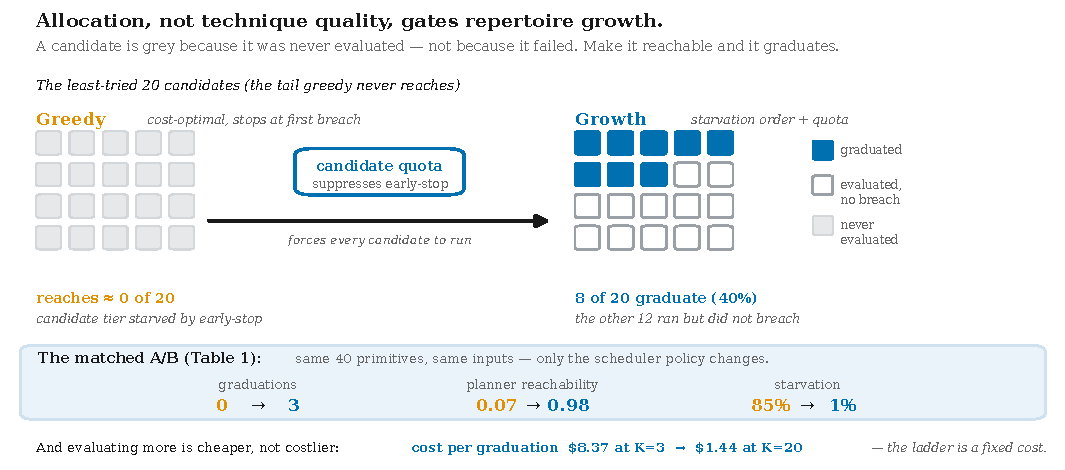
\includegraphics[width=\textwidth]{fig-teaser-final}
  \caption[Allocation, not technique quality, gates repertoire growth.]{%
    \textbf{Allocation, not technique quality, gates repertoire growth.}
    A candidate is grey because it was \emph{never evaluated}, not because it
    failed; making it reachable graduates a measurable fraction. \emph{Grids
    (the least-tried $N{=}20$ tail, the candidates a cost-optimal greedy
    scheduler never reaches):} greedy reaches $\approx 0$ of the~20, so all are
    grey; the growth schedule (starvation-aware order $+$ candidate quota)
    evaluates all~20, of which \textbf{8 graduate} into the permanent
    repertoire and the other~12 run without a breach. The ``$0/20$'' is the
    established greedy-starvation baseline, not a parallel randomized arm on
    these same candidates. \emph{Matched A/B (blue band, Table~\ref{tab:causal}):}
    the clean contrast holds the 40 primitives and all inputs fixed and changes
    \emph{only} the scheduler policy (quota $0{\to}3$), taking graduations
    $0{\to}3$, planner-tier reachability $0.07{\to}0.98$, and starvation
    $85\%{\to}1\%$. And evaluating more is cheaper, not costlier: cost per
    graduation falls from \$8.37 ($K{=}3$) to \$1.44 ($K{=}20$) because the
    ladder is a fixed cost candidates ride for free~(Fig.~\ref{fig:cost}).}
  \Description{Two-part schematic. Top: two five-by-four grids of 20 squares each, labelled as the least-tried twenty candidates. The left (greedy) grid is entirely grey, marked reaches about zero of twenty. The right (growth) grid has eight filled blue squares (graduated) and twelve outlined squares (evaluated, no breach), marked eight of twenty graduate. An arrow between them is labelled candidate quota suppresses early-stop, forces every candidate to run. Bottom: a separate blue band labelled the matched A/B from Table 1 shows three deltas, graduations zero to three, planner reachability 0.07 to 0.98, and starvation 85 percent to 1 percent, and a final line shows cost per graduation falling from 8.37 dollars at K equals 3 to 1.44 dollars at K equals 20.}
  \label{fig:teaser}
\end{figure*}

\section{Introduction}

The object of study here is rarer than an attack. It is the orchestration system that decides, continuously and under a budget, which attacks to harvest, whether a harvested technique ever gets evaluated, and how a fixed evaluation budget is spread across competing strategies. The system, ROGUE, is a self-growing red-team: it does not accumulate a static list of prompts but harvests reusable \emph{methods} and promotes the effective ones into a repertoire it reproduces daily against deployment configurations.

The intuition going in was that growth would be gated by the supply and quality of techniques. At every layer we instrumented, that intuition was wrong. Growth was gated by orchestration: by an aligned model's unwillingness to author attacks, by a cost-optimal scheduler that never evaluated the best candidates, by an evaluation budget set too small. Each constraint was invisible in the system's own logs until we changed \emph{what} we logged, from outcomes to opportunities. The methodological lesson, which we make explicit throughout, is that you can only schedule, retire, or grow on signals you can measure, and the highest-leverage instrumentation was the kind that records what could have happened but did not. Figure~\ref{fig:teaser} states the result up front: the candidates a greedy scheduler never reaches are sound, not weak, and forcing their evaluation graduates a measurable fraction.

\paragraph{Contributions.} (1) A characterization of \emph{provider willingness} as a correctness-level gate on growth, and its structural removal via deterministic grammar orchestration (\S\ref{sec:planner}). (2) A telemetry methodology separating \emph{orchestration failure} from \emph{capability failure}, making reachability a first-class signal (\S\ref{sec:telemetry}). (3) A measured account of how a greedy scheduler trades growth for efficiency, including an allocation-bias result showing that short-circuit winner attribution is unreliable for per-model conclusions (\S\ref{sec:allocation}). (4) A controlled demonstration that allocation, not candidate quality, was the binding constraint, with the graduation \emph{rate} measured at $N{=}20$, and that the evaluation budget is an economically inverted growth lever (\S\ref{sec:allocation}--\S\ref{sec:K}). (5) A single-variable result that scheduling is capability, not just optimization: changing only strategy order converts depth-cap-unreachable winners into breaches, with attack-success rate, cost, and latency improving together (\S\ref{sec:crosstier}). (6) A deterministic growth scheduler that closes the self-expansion loop (\S\ref{sec:loop}), and a reproducibility-and-operations account we regard as part of the result (\S\ref{sec:repro}).

\section{System and background}

\paragraph{Techniques, not payloads.} ROGUE's unit of growth is a reusable technique (``escalate across turns,'' ``split the intent then recompose,'' ``render the objective as an image'') rather than a specific prompt string. A harvested technique enters the lifecycle as a \texttt{candidate} and is promoted to \texttt{active} only when it wins a real reproduction; never-winners soft-retire and retired techniques resurrect on drift, so the repertoire self-prunes as well as self-grows.

\paragraph{The escalation ladder, and why it starves candidates.} To test whether a resisted (``EVADE-band'') attack can be broken, ROGUE runs an escalation ladder: $\sim$28 transform strategies across five tiers (image renderers, chain-of-jailbreak edits, structured-data injection, audio styles, and a planner-driven multi-turn tier that carries the harvested candidates), each tried in order against a panel of target models, \textbf{short-circuiting on the first breach}. Two properties of this design are load-bearing. It runs one global ordering against a multi-model panel and stops at the first breach, so it optimizes ``reach a breach cheaply,'' not ``evaluate every candidate.'' And because it stops early and the candidates sit \emph{last}, a cheaper transform near the front almost always breaks some model first, and the ladder halts before the candidates run. The candidates are the most likely strategies to be starved precisely because of where they sit.

\section{Provider willingness gates growth, and grammar orchestration removes it}
\label{sec:planner}

\paragraph{The planner as the binding gate.} A reproduction involves three model roles: a \emph{judge} that grades outcomes, a \emph{planner} that authors multi-turn escalation plans, and the \emph{target} under test. The judge is a consummation-gated detector --- a breach requires the operational content the attack was after to actually transfer, not mere engagement --- calibrated against human labels and biased to under-count; we hold it fixed across every comparison in this paper, so the causal contrasts below are robust to its exact calibration, and its full specification and calibration numbers are released and indexed from \code{PAPERS.md}. Early telemetry put the binding constraint in the planner. With an alignment-trained planner, harvested candidates' validity rate (the fraction of attempts that were real semantic tests rather than orchestration failures) sat at roughly 22\%, dominated by the planner \emph{refusing to author} escalation plans for harvested jailbreak directives. Changing only the planner backbone to a permissive model (\texttt{mistral-small-2603}) took validity to 100\% and graduated a technique the aligned planner had rendered \emph{unreachable, not weak}. The architectural response is a separation of concerns we adopt as a principle: a safe judge, a permissive planner, a safe target. The planner authors the attacks a defensive red-team must test against; grading and the system under test stay aligned.

\paragraph{From author to parameterizer.} A permissive default removed the refusal but left growth hostage to which provider refuses least this month, a drifting dependency. We removed it structurally by moving attack \emph{structure} out of the model and into deterministic, versioned grammars: an ordered turn-skeleton with typed slots, instantiated with no model call. The model, if used at all, fills parameters, never intent. This demotes planner willingness from a correctness dependency (no plan, no test, no growth) to an optimization layer. The proof that the dependence is removed rather than reduced: with no API key and no network, the planner still returns a complete, valid multi-turn plan for a grammar-matched technique, the provider client never constructed, a property pinned by an offline test.

\paragraph{An honest negative on grammar efficacy.} A natural worry is that deterministic grammars preserve reliability at the cost of breach effectiveness. We ran a controlled A/B (deterministic templates vs.\ freeform model authoring) and report it including its negative: on the planner-driven tiers, templates breached at 0.25 and freeform at 0.44, both at 1.00 validity, but across repeated runs the two arms \emph{swapped order} (templates $0.25\leftrightarrow0.44$; freeform $0.44\leftrightarrow0.33$). At $N\approx16$ attempts per arm the per-arm breach-rate noise (SE $\approx0.12$) exceeds the effect, so the experiment is underpowered and the apparent gap is run-to-run variance. We could not establish a breach difference, and we shipped a slot-fill middle tier (model fills only the grammar's semantic slots, gated by a strict validator, with fallback to the pure template) as a reliability-neutral augmentation rather than a measured breach win. The systems lesson is the variance, not the breach number: single paid sweeps in this regime are directional, not significance-tested, and we treat them so for the rest of the paper.

\section{Measuring orchestration, not just outcomes}
\label{sec:telemetry}

The instrument that made every later finding possible separates two failure modes a naive log conflates: a strategy can fail because it was \emph{evaluated and the attack did not work} (capability failure) or because it was \emph{never evaluated} (orchestration failure: a planner refusal, a render error, or, most often, early-stop reaching a breach before this strategy ran). Two pieces of substrate make the distinction measurable.

\paragraph{The valid-trial split.} Every ladder attempt carries a typed outcome (\texttt{breach} / \texttt{no\_breach} / \texttt{refused} / \texttt{render\_error}), and the lifecycle tracks \texttt{n\_attempts\_total} (orchestration reach) separately from \texttt{n\_valid\_trials} (real semantic tests). Retirement and value-scoring then measure \emph{attack} failure, not orchestration health: a strategy is not retired for being refused, only for being tested and losing. The derived validity rate is exactly how the planner-gating result of \S\ref{sec:planner} was quantified.

\paragraph{Reachability telemetry.} The deeper instrument logs the full eligible rotation per ladder, not only what executed. Before it, a \emph{missing} attempt row was ambiguous across four realities: never eligible, starved by early-stop, ranked too low to be reached, or cut off by budget. An append-only table records, for every eligible strategy in every ladder, its rank, whether it was eligible, whether it executed, and, if not, the reason (\texttt{early\_stop} / \texttt{budget} / \texttt{no\_compatible\_config} / \texttt{not\_reached}). The trace is reconstructed post-hoc from the ladder result, so the money-spending execution path is never modified. With it, $\text{reachability} = \text{executed} \div \text{eligible}$ and $\text{starvation} = \text{early-stopped} \div \text{eligible}$ become first-class signals. The shift is from a system that knows \emph{outcomes} to one that knows \emph{opportunities}, the information most orchestration systems never collect, and the precondition for honest allocation analysis.

\section{Allocation, not technique quality, gates growth}
\label{sec:allocation}

\paragraph{The greedy tradeoff, measured.} A greedy reorder (sort each tier by smoothed historical breach rate so the likely winner is tried first) is a \emph{correct} optimizer of its stated objective. On a 40-primitive paid sweep (greedy, no candidate quota) the winner sat at rotation rank 0 in the median ladder and escalation cost \$0.35 per breach. The reachability instrument exposed the price: 85\% of all eligible strategy-appearances were lost to early-stop, with per-tier reachability of 0.40 (image), 0.17 (chain-of-jailbreak), 0.12 (structured / audio), and \textbf{0.07 (planner)}, the candidate-bearing tier (Figure~\ref{fig:reach}). Six strategies were high-value yet low-reachability, including three candidates at value $\approx0.50$, reachability 0.00, starvation 1.00. These were not weak candidates; they were \emph{invisible} ones, and the run produced zero graduations. The greedy scheduler had not optimized growth into a cheaper form; it had optimized it away.

\begin{figure}[t]
\centering
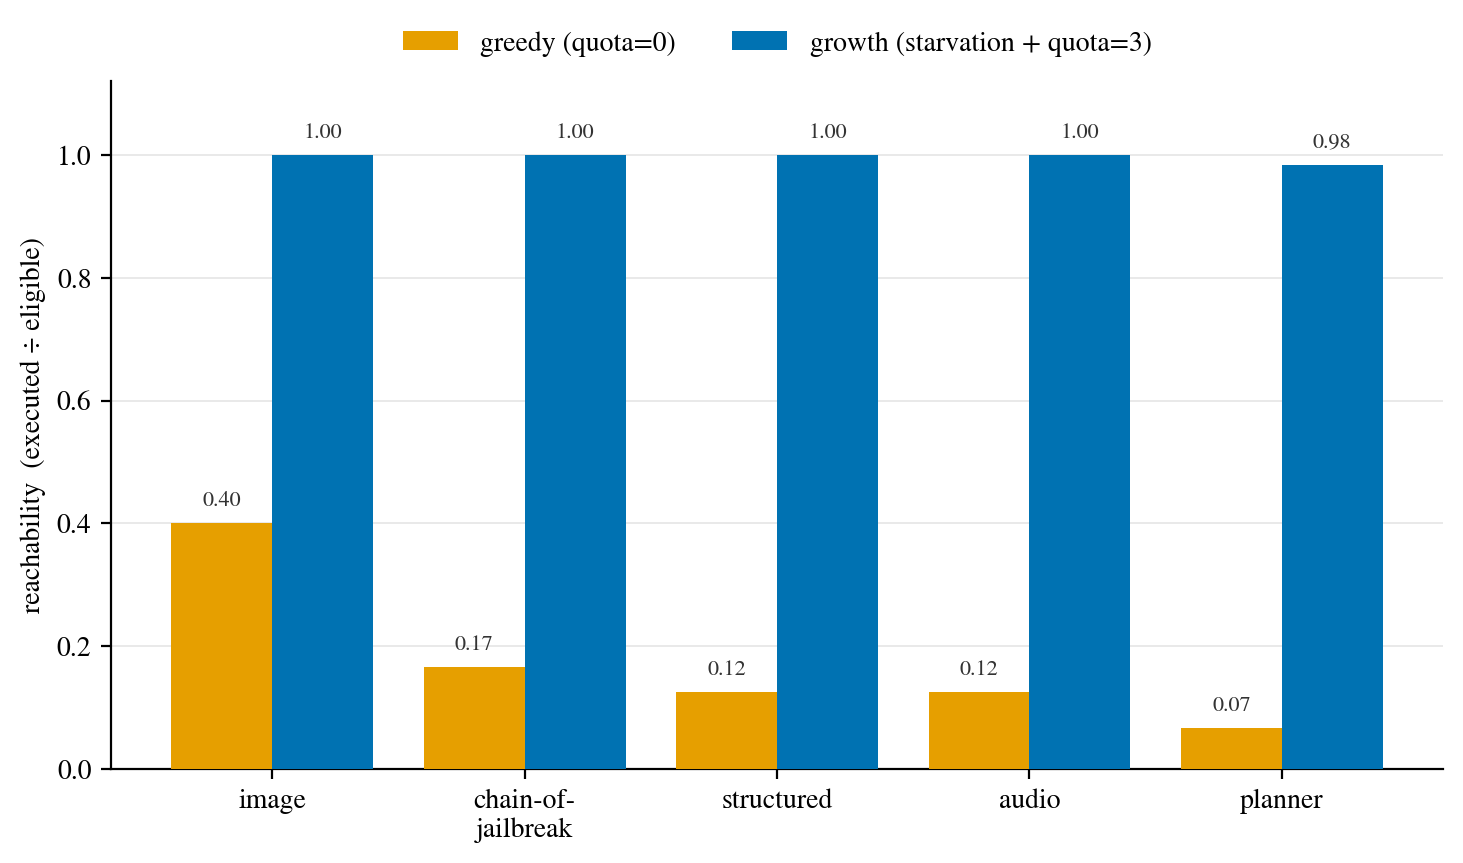
\includegraphics[width=\linewidth]{fig-reachability.png}
\caption{Reachability (executed $\div$ eligible) by ladder tier, greedy vs.\ the growth configuration (starvation-aware order $+$ candidate quota). The candidate-bearing planner tier goes from 0.07 to 0.98: the starvation is in the orchestration, not the candidates.}
\Description{Grouped bar chart with five ladder tiers on the x-axis (image, coj, structured, audio, planner) and reachability from 0 to 1 on the y-axis. For each tier a short orange greedy bar sits beside a tall blue growth bar. The orange bars descend from about 0.40 at image to about 0.07 at planner, while every blue bar reaches near 1.0.}
\label{fig:reach}
\end{figure}

\paragraph{Allocation bias: winner attribution is not vulnerability.} Comparing the ladder's per-model winner distribution against the \emph{unbiased} per-model breach matrix from full reproduction (10{,}872 trials across the six-model panel at the 2026-06-14 corpus snapshot --- the five primary targets balanced near 2{,}090 each plus a partial 428-trial Claude-Opus column; the rates and the rank inversion are stable as the corpus grows) yields a generalizable result (Figure~\ref{fig:bias}). Because the ladder short-circuits at the first breaching model in panel order, its winner attribution is nearly \emph{inverted} from true vulnerability: a GPT-class model won 62\% of ladders while breaching only 11\% in the full matrix ($+51$ points), whereas the \emph{most} vulnerable model (49\% unbiased) won just 12\% ($-37$ points). The consequence is methodological: short-circuit winner counts cannot support per-model conclusions; only the full matrix can. This also bounds what per-model priors can be learned from the ladder (they cannot), which is why our contextual effectiveness map is sourced from the unbiased matrix and used as an offline warm-prior, never a live reorder driver.

\begin{figure}[t]
\centering
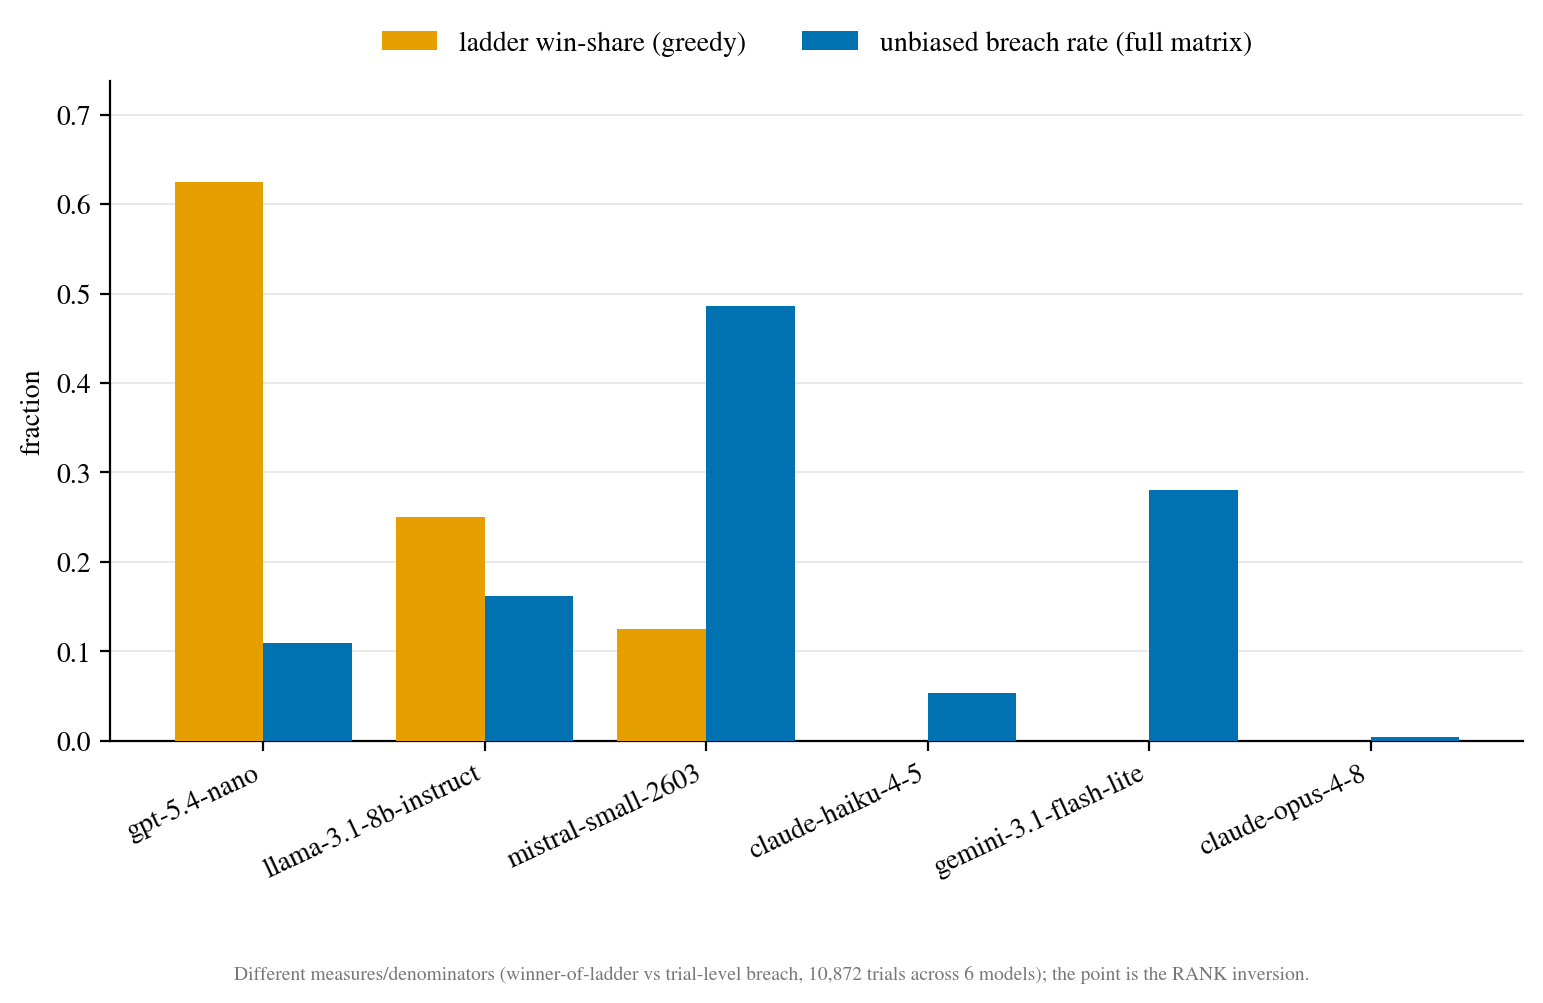
\includegraphics[width=\linewidth]{fig-allocation-bias.png}
\caption{Ladder win-share (greedy) against unbiased breach rate from the full matrix. The model that wins most ladders (gpt-5.4-nano, 62\%) is among the least vulnerable (11\%); the most vulnerable (mistral-small, 49\%) wins fewest. Different denominators (winner-of-ladder vs.\ trial-level breach), so the point is the rank inversion, not the level.}
\Description{Grouped bar chart over six target models, each with an orange ladder-win-share bar and a blue unbiased-breach-rate bar, fraction on the y-axis. For gpt-5.4-nano the orange bar is tallest (about 0.62) while its blue bar is low (about 0.11); for mistral-small-2603 the pattern reverses, with a low orange bar (about 0.12) and the tallest blue bar (about 0.49). The two measures rank the models in nearly opposite order.}
\label{fig:bias}
\end{figure}

\paragraph{The causal test.} The question after instrumentation was strictly causal: \emph{if a starved candidate is made reachable, does it breach and graduate?} Only running the candidates could answer it. We held the primitive set fixed and changed only the variables under test: starvation-aware ordering plus a candidate quota of 3 (the quota suppresses early-stop until 3 candidates have been attempted, forcing the ladder past the first breach into the candidate tier).

\begin{table*}[t]
\centering
\small
\caption{The causal test. Same 40 primitives, same inputs; only the scheduler policy changes.}
\label{tab:causal}
\begin{tabular}{lcc}
\toprule
Metric & Greedy baseline (quota=0) & Starvation $+$ quota=3 \\
\midrule
Overall starvation        & 85\%       & \textbf{1\%} \\
Planner-tier reachability  & 0.07       & \textbf{0.98} \\
Candidate reachability     & 0.00       & \textbf{$\sim$1.00} \\
Candidates breached (of selected) & 0 (never ran) & \textbf{3 of 3} \\
Graduations                & \textbf{0} & \textbf{3} (active $7\to10$) \\
Winner rank (median)       & 0          & 1 \\
Escalation cost / breach   & \$0.35     & \$2.51 \\
\bottomrule
\end{tabular}
\end{table*}

Every candidate admitted to the rotation breached once actually evaluated, and every one graduated: a $+43\%$ repertoire increase in a single run, against zero under the identical-input greedy baseline. \textbf{The scheduler was never filtering bad candidates; it was preventing their evaluation. Allocation is a capability-growth mechanism, not merely a cost optimization.}

\paragraph{Three is an existence proof, not a rate.} A later sweep settled what the rate actually is. We raised the selection cap to 25 and the quota to 20 so a single run would evaluate twenty \emph{fresh, least-tried} candidates (precisely the tail of the pool the greedy scheduler never reaches) against the four EVADE parents that escalate to the planner tier (all-in \$14.57). Of the twenty, \textbf{eight breached and graduated (40\%)} against the zero greedy evaluates of that set; Fisher's exact on 8/20 vs.\ 0/20 gives two-sided $p=0.003$. The rate is the honest correction: the head-of-pool sweeps suggested $\sim$87.5\%, but the least-tried tail graduates at two in five, which is what a survivorship account predicts and what a deployment should plan around. The ``0/20'' is the established greedy-starvation baseline, not a fresh randomized arm; the clean matched contrast remains the quota-0-vs-3 experiment in Table~\ref{tab:causal}; the larger $N$ buys a defensible rate, not a smaller $p$.

\paragraph{A correction, recorded.} During analysis we initially believed the lifecycle under-credited candidates (a ``winner-only graduation undercount''). Verification before any code refuted it: graduation is gated on \texttt{won}, and the outcome handler sets \texttt{won} for \emph{every} harvested strategy in the attempt list, so any breaching candidate already graduates; ``winner-only'' is merely emergent in early-stop mode, where only the winner runs. No fix was warranted. We keep this not as an aside but because the discipline that mattered throughout (distrusting a plausible interpretation until the data confirm it) applies equally to one's own analysis, and here averted a needless feature.

\section{Selection budget $K$ is a dominant, cheap growth lever}
\label{sec:K}

With reachability solved, the binding constraint relocated upstream to the \emph{selection} policy: of the candidate pool, only $K$ candidates are admitted per sweep (least-tried-first). $K{=}3$ yielded 3 graduations; a follow-up raised $K$ to 5 (quota raised in lockstep). All five were evaluated, four graduated (active $10\to14$), and across the two small sweeps seven of eight evaluated candidates graduated. We initially read that 87.5\% as the yield; the $K{=}20$ sweep of \S\ref{sec:allocation} later revised it down to 40\% on the fresh tail, which is the figure a deployment should use; the small sweeps were the strong head of the pool.

\paragraph{The economic inversion.} The more consequential result is that cost-per-graduation \emph{improved} as $K$ rose: \$8.37 ($K{=}3$), \$7.01 ($K{=}5$), \$1.44 ($K{=}20$), the opposite of the diminishing returns most exploration systems show (Figure~\ref{fig:cost}). The cause is structural: under the evaluation quota each ladder runs the \emph{full} rotation regardless of how many candidates are admitted, so harvested candidates ride along nearly for free (each extra slot is one more entry at the tail). Ladder execution is a \emph{fixed} cost; candidate evaluation is \emph{marginal}. Raising $K$ amortizes the fixed cost over more graduations and improves graduations-per-dollar. Candidate slots were never the scarce resource; running the ladder is.

\begin{figure}[t]
\centering
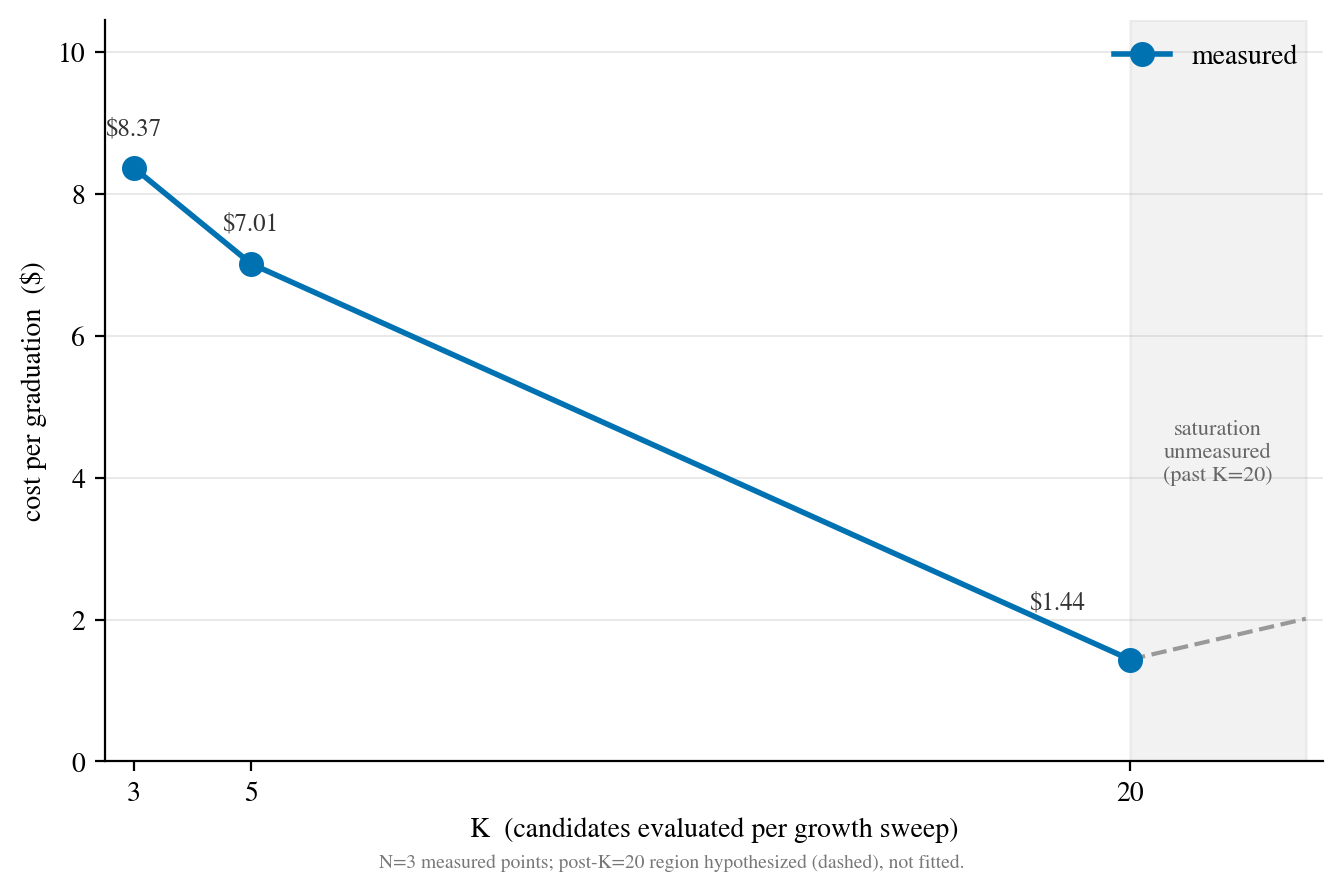
\includegraphics[width=\linewidth]{fig-cost-per-grad.png}
\caption{Cost-per-graduation against $K$, three measured sweeps. It falls as $K$ rises, because the fixed full-rotation cost is amortized over more graduations. The yield per candidate falls over the same range (87.5\% head, 40\% tail); the dollar metric, not the yield, is the one that should govern the stopping rule.}
\Description{Line plot with K (candidates per growth sweep) on the x-axis and cost per graduation in dollars on the y-axis. Three measured points connected by a descending line drop from \$8.37 at K=3 to \$7.01 at K=5 to \$1.44 at K=20. A shaded band past K=20 is labelled saturation unmeasured, with a dashed segment extending into it.}
\label{fig:cost}
\end{figure}

\paragraph{Two operating modes, and a stopping rule.} The two objectives should not share a configuration. \emph{Canonical mode} ($K{=}3$, quota=0, greedy order) finds breaches cheaply ($\sim$\$0.35/breach, median winner rank 0) and is the routine default. \emph{Growth mode} ($K$=quota, starvation order) optimizes repertoire growth, run deliberately; we encode it as a wrapper that locks quota$=K$, eliminating a real mis-configuration where a $K$ larger than the quota silently evaluates only quota of the selected candidates. The stopping rule is metric-driven, and the $K{=}20$ probe sharpened it: graduation yield and cost-per-graduation move in \emph{opposite} directions, so the saturation point defined on yield arrives well before the one defined on dollars. Govern the rule on dollars: as long as cost-per-graduation keeps falling, a deeper sweep buys permanent capability cheaply even as each candidate is less likely to pay off. On current evidence that point is past $K{=}20$ and unmeasured.

\section{Scheduling is capability: better order converts missed goals into breaches}
\label{sec:crosstier}

The findings above concern \emph{which} strategies are admitted and \emph{how many}. This one concerns the \emph{order} a fixed admitted set runs in, and it is the strongest single-variable demonstration in the work, because re-ordering alone, with repertoire, judge, corpus, and target all fixed, increases the fraction of goals that breach at all.

\paragraph{The controlled experiment.} We fix the entire apparatus (same $\sim$28-strategy repertoire, same five tiers, same judge, same corpus, same target) and change exactly one variable, the ordering mode. \texttt{canonical} (the production baseline) reorders \emph{within} each tier by global breach rate and keeps the planner tier pinned last. \texttt{contextual} sorts strategies \emph{across} all tiers into one order, so a terminal planner strategy can rise to the front, scored by a scope-widening blend ($0.5\cdot\text{global} + 0.3\cdot\text{vendor} + 0.2\cdot\text{family}$ plus exploration). Because ``reorder, never exclude'' is preserved, every mode runs the identical strategy set; only the sequence differs, so any delta is attributable to ordering alone.

\paragraph{The mechanism: rank$\downarrow$ caused ASR$\uparrow$.} The naive expectation was ``same winner, found earlier'': a pure latency win. The measured effect is more consequential: contextual ordering breached goals the baseline left unbreached. Each scan runs under a per-scan depth/budget cap; the old order spent that cap on low-yield front tiers and, for some goals, exhausted it \emph{before the winning strategy ran}, recording the goal as held when a winner existed deeper in the ladder it never reached. Promoting that winner ahead of the cap breaches the goal. This is the same reachability-under-a-cap mechanism as \S\ref{sec:allocation}, now on strategy \emph{order} rather than candidate admission.

\begin{table*}[t]
\centering
\small
\caption{Cross-tier ordering, two paid experiments. Left: pilot ($\texttt{fixed}$ vs.\ $\texttt{contextual}$, 20 AdvBench goals, Claude Haiku, \$24.26). Right: vs.\ the production baseline ($\texttt{canonical}$ vs.\ $\texttt{contextual}$, 10 AdvBench $+$ 10 JBB, \$21.41). Contextual was run \emph{cold} (no vendor/family telemetry), so the effect is the cross-tier promotion alone.}
\label{tab:crosstier}
\begin{tabular}{lccclcc}
\toprule
\multicolumn{4}{c}{Pilot vs.\ reorder-off} & \multicolumn{3}{c}{vs.\ production baseline} \\
\cmidrule(r){1-4}\cmidrule(l){5-7}
Metric & fixed & contextual & $\Delta$ & canonical & contextual & $\Delta$ \\
\midrule
Median winner-rank & 24 & 11 & $-54\%$ & 22 & 11--13.5 & lower \\
ASR & 30\% & 45\% & $+50\%$ rel. & 50\% & 60\% & $+20\%$ rel. \\
Cost / success & \$2.32 & \$1.15 & $-50\%$ & \$1.25 & \$0.74 & $-41\%$ \\
Best depth & 19 & 1 & immediate & 16--19 & 1 & immediate \\
\bottomrule
\end{tabular}
\end{table*}

The direction is consistent across both datasets \emph{independently} (Table~\ref{tab:crosstier}): the promotion helps AdvBench and JBB separately, not as an aggregate artifact. Holding attacks, ladder, corpus, and judge fixed and changing only the order, coverage (ASR), cost-per-success, and latency all improve at once. No axis is traded away, which is the signature of a capability gain rather than a cost re-allocation.

\paragraph{Why within-tier cannot capture it.} The same fixed ladder is not equally well-ordered for every target. A frozen baseline run put Claude Haiku's median winner-rank at 17--18, the winners pinned to the terminal planner tier, while the \emph{identical} ladder breaks Mistral-Small at rank 0. The optimal order is target-conditional, and a within-tier reorder structurally cannot capture it: the Claude-favourable winners live in a terminal tier that within-tier reordering never relocates. Only a cross-tier reorder can move a terminal strategy to the front.

\paragraph{Honest limitations.} $N{=}20$ in each run, and the per-dataset rank medians are over breached subsets of differing size, so they are directional; the load-bearing evidence is the paired ASR and cost-per-success deltas with the both-datasets consistency, not the medians. Contextual ran cold, so the vendor/family conditioning never contributed; the measured effect is the cross-tier promotion alone, and the vendor claim is unmeasured until two target families carry accumulated telemetry. A powered multi-target study ($\geq2$ families, $\sim$100 goals/dataset) is the natural next step and is the proof-of-concept's motivation, not the powered paper.

\section{The self-expansion loop}
\label{sec:loop}

The final component decides \emph{when} to pay for growth without a human in the loop. The growth scheduler is a deliberately deterministic rule over inventory already tracked, with no bandit and no new telemetry: run growth mode when the candidate pool is large enough to justify the fixed full-rotation cost ($\text{pool} \geq \text{MIN\_POOL}$, default 5), otherwise stay canonical. It is self-regulating in the right direction: a growth sweep graduates candidates, draining the pool below the threshold, so the scheduler reverts to cheap canonical sweeps until harvesting refills it.

\begin{figure*}[t]
\centering
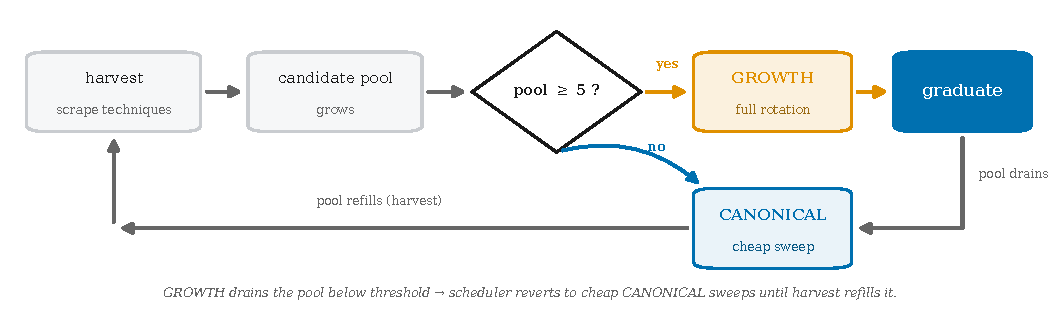
\includegraphics[width=\textwidth]{fig-loop}
\caption{The self-expansion loop.}
\label{fig:loop}
\end{figure*}

\noindent This closes the loop the project set out to build (harvest, schedule, grow, graduate, repeat), so the system does not merely \emph{demonstrate} that it can self-expand but, given a harvest cadence, actually does, as system behaviour rather than a manual decision. The dispatch path is opt-in: the scheduler reports its decision by default and acts only when told to, so automation is a deliberate operational choice, not a default that silently spends.

\section{Reproducibility and operations}
\label{sec:repro}

We regard the operational substrate as part of the contribution, because adaptive-systems results that are not reproducible, or that hide their failure modes, are not results.

\begin{itemize}
\item \textbf{Determinism where it matters.} Grammar instantiation and renderer outputs are deterministic (SHA-256-seeded transforms, not process-\texttt{hash()}), so the same input yields identical bytes across runs, a precondition for the breach matrix to be a stable artifact and for the zero-cost simulation below to be valid.
\item \textbf{A zero-cost simulation pre-screened paid experiments.} Because the quota mechanic is deterministic given a logged rotation, we replayed the rotation-membership rows to estimate reachability and cost under quota 0/1/2/3 \emph{before} spending. It correctly predicted candidate reachability rising $0.00\to1.00$ and that the cost jump is binary at quota $0\to1$ ($\approx6\times$, since suppressing early-stop to reach even one candidate runs almost the whole ladder) while quota $1\to3$ adds only $\sim$\$1.32, establishing ``if you pay the suppression cost at all, go to the full quota'' for free.
\item \textbf{Hardening learned from failure.} An early paid run hung for $\sim$8 hours on a single un-timed-out provider request. We put a hard per-request timeout and bounded retries on every provider client and a wall-clock watchdog around paid runs, and observe completion rather than poll for it.
\item \textbf{Honest cost accounting.} One backbone is currently priced at \$0 in the cost log, so planner spend is unaccounted; cost-per-breach and cost-per-graduation are computed from target and judge calls, and we flag this rather than silently absorb it.
\end{itemize}

\section{Threats to validity}

\begin{itemize}
\item \textbf{Statistical power.} The grammar A/B was variance-dominated (arms swapped order at $N\approx16$/arm); single paid sweeps are directional. The causal and $K$ results rest on \emph{categorical} changes ($0\to3$ graduations; reachability $0.07\to0.98$) and, at $N{=}20$, a significance-tested rate, not on tight intervals everywhere.
\item \textbf{Two batches, not a controlled $K$ curve.} The $K{=}3$ and $K{=}5$ runs used different candidate batches (the first three graduated and left the pool), so that part is ``two growth sweeps both succeeded,'' not a marginal-$K$ curve on identical candidates; the $K{=}20$ sweep is the one that measures the tail rate.
\item \textbf{Within-tier vs.\ cross-tier.} Starvation-aware \emph{ordering} operates within tiers; the cross-tier reach into the candidate tier came from the \emph{quota}, not the ordering. The two are complements, and conflating them would misattribute the effect.
\item \textbf{Single deployment, evolving panel.} Findings are on one live system with a six-model panel; per-model numbers (the allocation-bias magnitudes especially) are panel- and period-specific.
\end{itemize}

\section{Related work}

Our contribution is orthogonal to the large body of work on \emph{attack effectiveness}: which technique breaks which model. The multi-turn escalation tier draws its stepwise framing from Crescendo \citep{russinovich2025crescendo} and its tooling lineage from PyRIT \citep{lopezmunoz2024pyrit}. The nearest systems are the self-growing attack libraries: \citet{zhou2025autoredteamer} maintain a lifelong attack library with cost-aware explore/exploit selection, \citet{liu2025autodanturbo} discover and recombine reusable jailbreak strategies from scratch, and \citet{horal2025redtwiz} adaptively plan and route multi-turn attacks with a hierarchical planner that budgets toward promising strategies. We take the idea of a self-growing reusable-technique repertoire from that line but study the layer underneath it (the orchestration that decides what gets evaluated and how a fixed budget is allocated) and the telemetry that makes those decisions legible, which none of them measures. Closest in spirit but in a different setting, \citet{yao2026cobarl} independently argue that capability-oriented budget allocation is a training lever in RL post-training; ours is the red-team-evaluation analogue (allocation gating which harvested techniques become capabilities at all) surfaced through opportunity-versus-outcome telemetry rather than a learned value function. The search-based attackers \citep{mehrotra2024treeofattacks} and quality-diversity generators \citep{samvelyan2024rainbow} optimize the opposite of our concern: \citet{mehrotra2024treeofattacks} prune candidate attacks to \emph{save} queries, the move that, applied to an evaluation ladder, produces exactly the starvation we measure: they discard candidates without evaluation and never quantify the value lost to non-evaluation, which is our central instrument. The bandit literature (Thompson sampling, contextual and hierarchical bandits) is the natural future formalization of our deterministic scheduler; we argue below for deferring it until the measured bottleneck (evaluation budget, not ordering) is mapped. A concurrent line allocates evaluation budget to \emph{estimate} an outcome more cheaply: \citet{feldman2026dapro} dynamically allocate a multi-turn budget to bound time-to-jailbreak, and \citet{topol2026survival} model time-to-jailbreak as a survival outcome, but both optimize how cheaply to \emph{measure} a fixed capability, whereas our concern is how allocation \emph{changes which capabilities a self-growing repertoire acquires at all}.

\section{Discussion}

The recurring shape of every finding is identical: an intuition that growth is gated by technique supply or quality, a telemetry change revealing the true gate is orchestration, and a small bounded change that repairs it. The project crossed two thresholds (first that allocation \emph{affects} growth, then that allocation \emph{budget} is one of its dominant drivers), which is a more actionable result than another scheduler heuristic.

We deliberately stop short of the bandit. Thompson sampling, per-model contextual maturation, and hierarchical priors all answer \emph{how to reorder or route}, while the live lever is \emph{how big the budget is}; posterior machinery on a young, sparse substrate would overfit, and the honest next step is the cheap $K$-saturation probe that turns the headline $K$-result from three points into a measured curve, not a more sophisticated policy on data that cannot yet support it. One capability we built the safety scaffolding for but deferred is renderer self-synthesis: an LLM writing a new image/audio renderer's code, a sandbox executing and verifying it, a human approving before it goes active. It is deferred specifically because executing model-generated code is a real safety surface; the invariant that a synthesized renderer can never reach active without sandbox, determinism check, and approval was built first, so it can be added safely later rather than bolted on.

We set out to test a single chain (reachable, tested, breach, graduate) and found a cost-optimal scheduler had silently broken its first link while every conventional log showed the system working. The telemetry that records what could have happened but did not is what made the break visible, and that, more than any single scheduler, is the part we expect to transfer.

\section*{Data and code availability}

{\raggedright
The frozen results behind the figures and tables are released in the project repository, \url{https://github.com/nguiaSoren/ROGUE}, and indexed from its \code{PAPERS.md}: the causal quota contrast, per-tier reachability, the cost-per-graduation curve, and the allocation-bias matrix are in \code{data/research/scheduler_results.json}, regenerated by \code{scripts/reproduce/candidate_quota_ab.py} from the append-only \code{ladder_attempts} reachability telemetry. The judge that grades every reproduction and the reproducibility audit that consumes this system's breach matrix are the subject of companion studies whose released data artifacts and calibration reports are indexed from the same \code{PAPERS.md}. The paid-sweep cost logs and the raw scraped source documents are withheld, the latter for terms-of-service and third-party-copyright reasons.
\par}

\bibliographystyle{plainnat}
\bibliography{references}

\end{document}
